\documentclass[hyperref={pdfpagelabels=true}]{beamer}%qnd referenciamos equação/figura etc o tex encaminha direto p pagina onde se encontra a equação.
\usefonttheme[onlymath]{serif} % fonte matematica
\setbeamersize{text margin left=0.4em,text margin right=0.2em,} % alterando as dimensões da página
\usepackage{enumerate}
\usepackage[utf8]{inputenc}
\usepackage{subfig}

\usepackage{pstricks,pst-node,pst-text,pst-3d}
\usepackage{amsfonts, amssymb, amsmath, amsthm, mathrsfs, times} %fontes
\usepackage[brazil]{babel}

%\usepackage{scalefnt} % escala de uma fonte, muda no próprio texto com barra alguma coisa.
% \usepackage{url}% permite entrar com uma URL e abre um navegador.
\usepackage[algoruled,longend]{algorithm2e}% escrever pseudo-códigos
\usepackage{algorithmic}
%\usepackage{multirow}
%\usepackage{subeqnarray}%subequações numeradas 1a,1b,....
%\usepackage[normalem]{ulem}%sublinhar
\usepackage{bbding} %para usar desenhos de mãos
\usepackage{bbm}
\usepackage{multimedia}

%propriedades do pacote algoritmo
%\renewcommand*{\listalgorithmcfname}{lista de algoritmos}  % altera o nome do indice
%\renewcommand*{\algorithmcfname}{Algoritmo}					% altera o nome do ambiente
%\renewcommand*{\algorithmautorefname}{algoritmo}			% não sei (testar)

\usepackage{color} 
\usecolortheme[RGB={25,0,254}]{structure}%para mudar a cor da apresentação
%\setbeamercolor {normal text}{bg= MyColor}  % Altera a cor do plano de fundo

\definecolor{MyBlue} {RGB}{100,100,255}   % Define uma nova cor
\definecolor{MyGrey} {RGB}{250,250,250}   % Define uma nova cor



%\newcommand{\bm}[1]{\boldsymbol{#1}}
%############################################
% Temas Padrões
%############################################
%\usetheme{AnnArbor}
%\usetheme{Antibes}
%\usetheme{Bergen}
%\usetheme{Berkeley}
%\usetheme{Berlin}
%\usetheme{Boadilla}
%\usetheme{boxes}
%\usetheme{CambridgeUS}
%\usetheme{Copenhagen}
%\usetheme{Darmstadt}
%\usetheme{default}
%\usetheme{Dresden}
%\usetheme{Frankfurt}
%\usetheme{Goettingen}
%\usetheme{Hannover}
%\usetheme{Ilmenau}
%\usetheme{JuanLesPins}
%\usetheme{Luebeck}
\usetheme{Madrid}
%\usetheme{Malmoe}
%\usetheme{Marburg}
%\usetheme{Montpellier}
%\usetheme{PaloAlto}
%\usetheme{Pittsburgh}
%\usetheme{Rochester}
%\usetheme{Singapore}
%\usetheme{Szeged}
%\usetheme{Warsaw}

% %% Mostrar o plano no inicio de cada seção
% \AtBeginSection[] 
% {
% \begin{frame}<beamer>
% \frametitle{Plano}
% \tableofcontents[currentsection]
% \end{frame}
% }%repete o slide do sumario cada vez q eh mudada a seção

%para alterar o rodapé da apresentação
\setbeamertemplate{footline}
{
\begin{beamercolorbox}{}%{section in head/foot}
\hskip4pt{\bf \insertshortauthor/\insertshorttitle/\insertshortdate} \hskip160pt {\insertframenumber/\inserttotalframenumber}
\vskip2pt\end{beamercolorbox}
}


% configurando o ambiente block
\setbeamertemplate{blocks}[rounded][shadow=true]  % ambiente block
\setbeamercolor{block title}{bg=MyBlue, fg = black}%bg=background, fg= foreground
\setbeamercolor{block body}{bg=MyGrey,fg=black}%bg=background, fg= foreground

%\useoutertheme{infolines}
\beamertemplatetransparentcovereddynamic% Deixa os item transparentes p/ aparecer um a um, desde que eu não aponte com o comando \pause
%\useoutertheme{tree}% Para ficar aparecendo o organograma do trabalho na parte superior do slide
%\usefonttheme{structurebold}
%\setbeamertemplate{footline}[frame number]% numera os slides
\setbeamertemplate{navigation symbols}{}%%% Elimina símbolos de navegação 
%\usepackage[tab]{beamerthemesidebar}% Coloca a barra lateral apontando os tópicos

%%% comandos para aparecer o logo em cada slide %%%
% \pgfdeclareimage[height=1.4cm]{logo}{v4}
% \logo{\pgfuseimage{logo}}

%\renewcommand{\insertdateindicator}{Evento}
\title[Reconstrução 3D]{Geometria Trifocal em Reconstrução 3D}
\author[David Pinho]{David da Costa de Pinho\\Orientador: Prof. Ricardo Fabbri, Ph.D}
\institute{IPRJ/UERJ} 
\date{}

% ************************************************************************
%		LISTA DE COMANDOS	
% ************************************************************************

\newcommand{\R}{\mathbb{R}}%substitui o comando grande apenas por R
\newcommand{\N}{\mathbb{N}}
\newcommand{\Z}{\mathbb{Z}}
\newcommand{\F}{\mathscr{F}}
\newcommand{\X}{\bf {X}}
\newcommand{\Y}{\mathcal{Y}}
\newcommand{\E}{\mathbb{E}}
\newcommand{\x}{{\bf x}}
\newcommand{\e}{{\bf e}}
\newcommand{\lightrgb}{{\bf l}}
\newcommand{\bpi}{\pi}
\newcommand{\y}{{\bf y}}


\theoremstyle{definition}
\newtheorem{teo}{Teorema}[section]


 %%%%%%%%%%%%%%%%%%%%%%%%%%%%%%%%%%%%%%%%%%%%%%%%%%%%%%%%%%%%%%%%%%%%%%%%%%%%%%
% Capa
%%%%%%%%%%%%%%%%%%%%%%%%%%%%%%%%%%%%%%%%%%%%%%%%%%%%%%%%%%%%%%%%%%%%%%%%%%%%%%

\begin{document}
\pgfdeclarelayer{background}
\pgfsetlayers{background,main}

\frame{%apara abrir cada slide
\thispagestyle{empty}%para nao aparecer numeração nem outros itens na pagina
  
\vspace{-.1cm}%subir ou descer a apresentação. com h vai p esquerda e direita

\begin{figure}
\centering
\subfloat{
\includegraphics[scale=0.37]{figuras/logo-uerj-2}}
\qquad
\subfloat{
\includegraphics[scale=0.3]{figuras/iprj}}
\vspace{1 cm}
\end{figure}  

\vspace{-1cm}
\maketitle
}
%
\frame{%\transwipe[direction=0]%forma de transição de slides
\frametitle{Sumário}
\tableofcontents%[pausesections]%puxa automaticamente cada seção criada
}
%
\section{Motivações}
\frame{\frametitle{Motivações}
%\begin{figure}
%\centering
%\subfloat{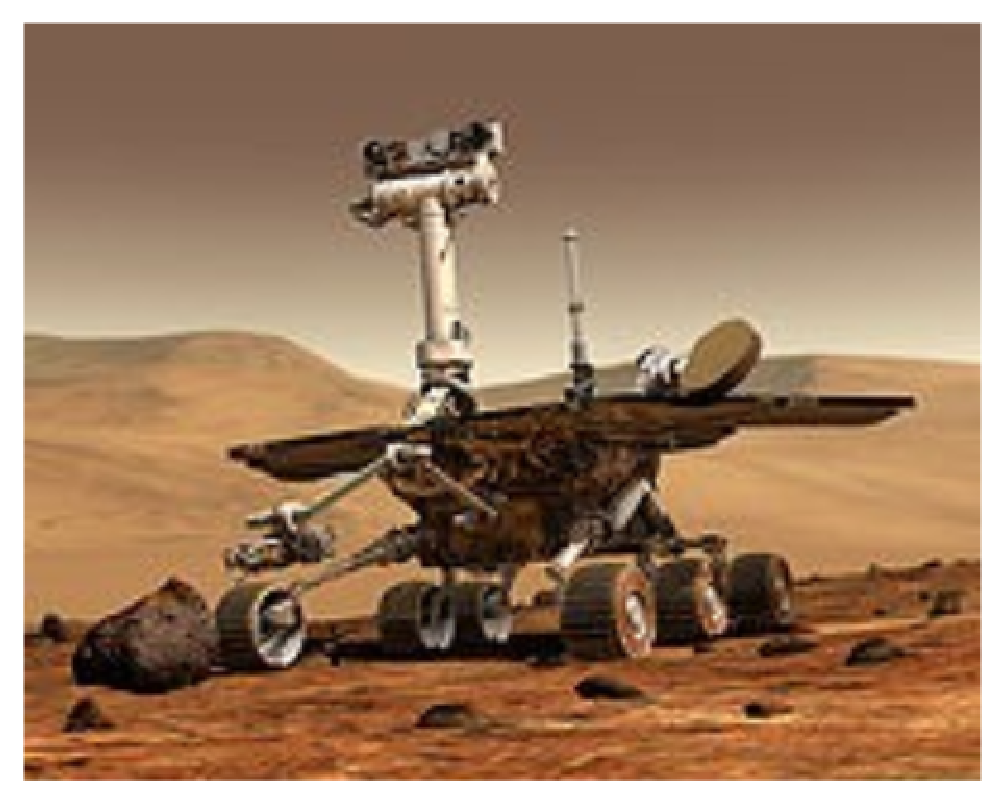
\includegraphics[scale=.23]{figuras/mars-rover}}
%\quad
%\subfloat{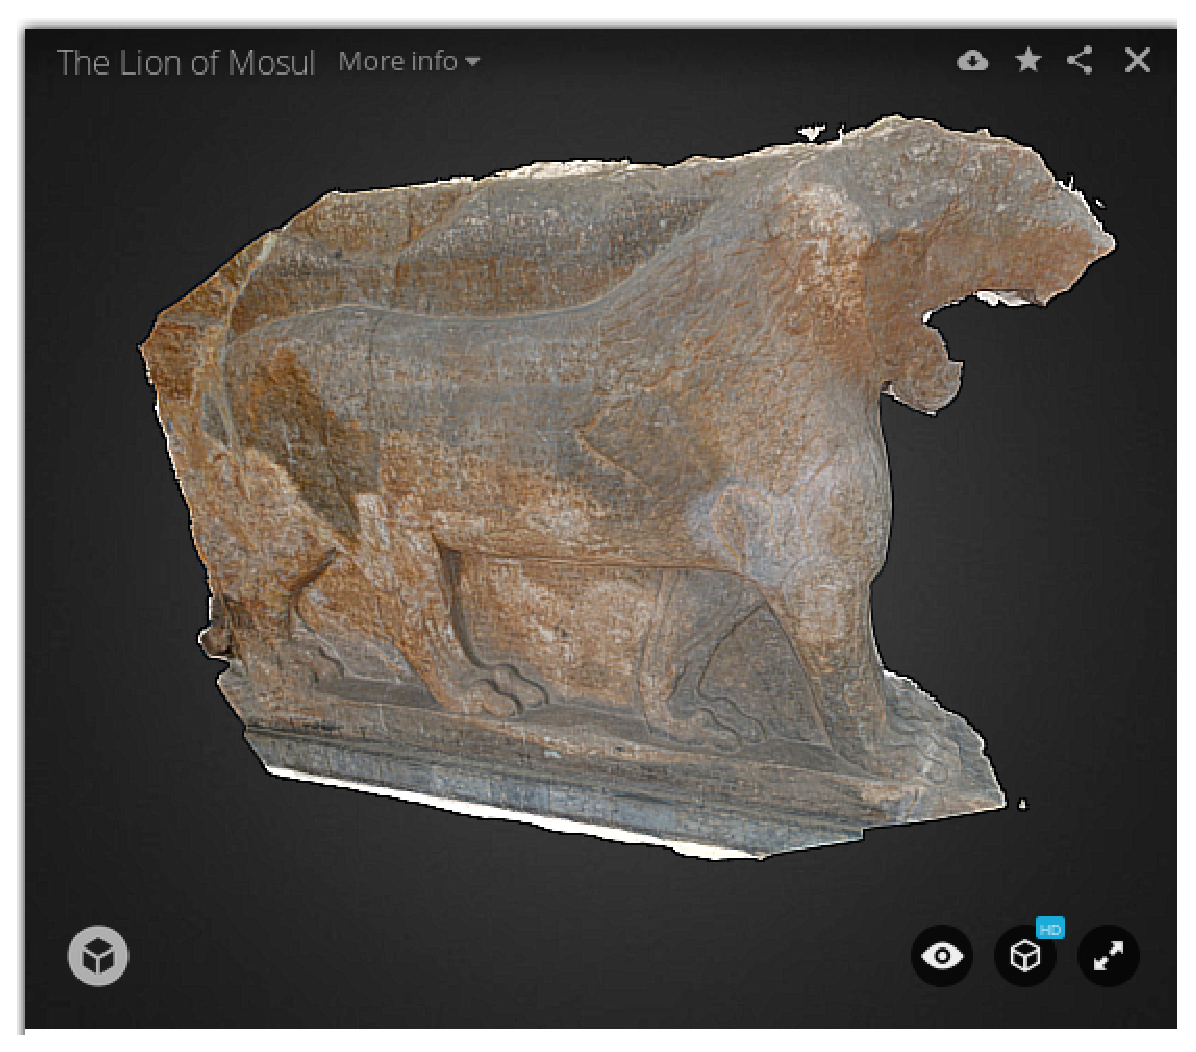
\includegraphics[scale=.18]{figuras/leao-mosul}}
%\quad
%\subfloat{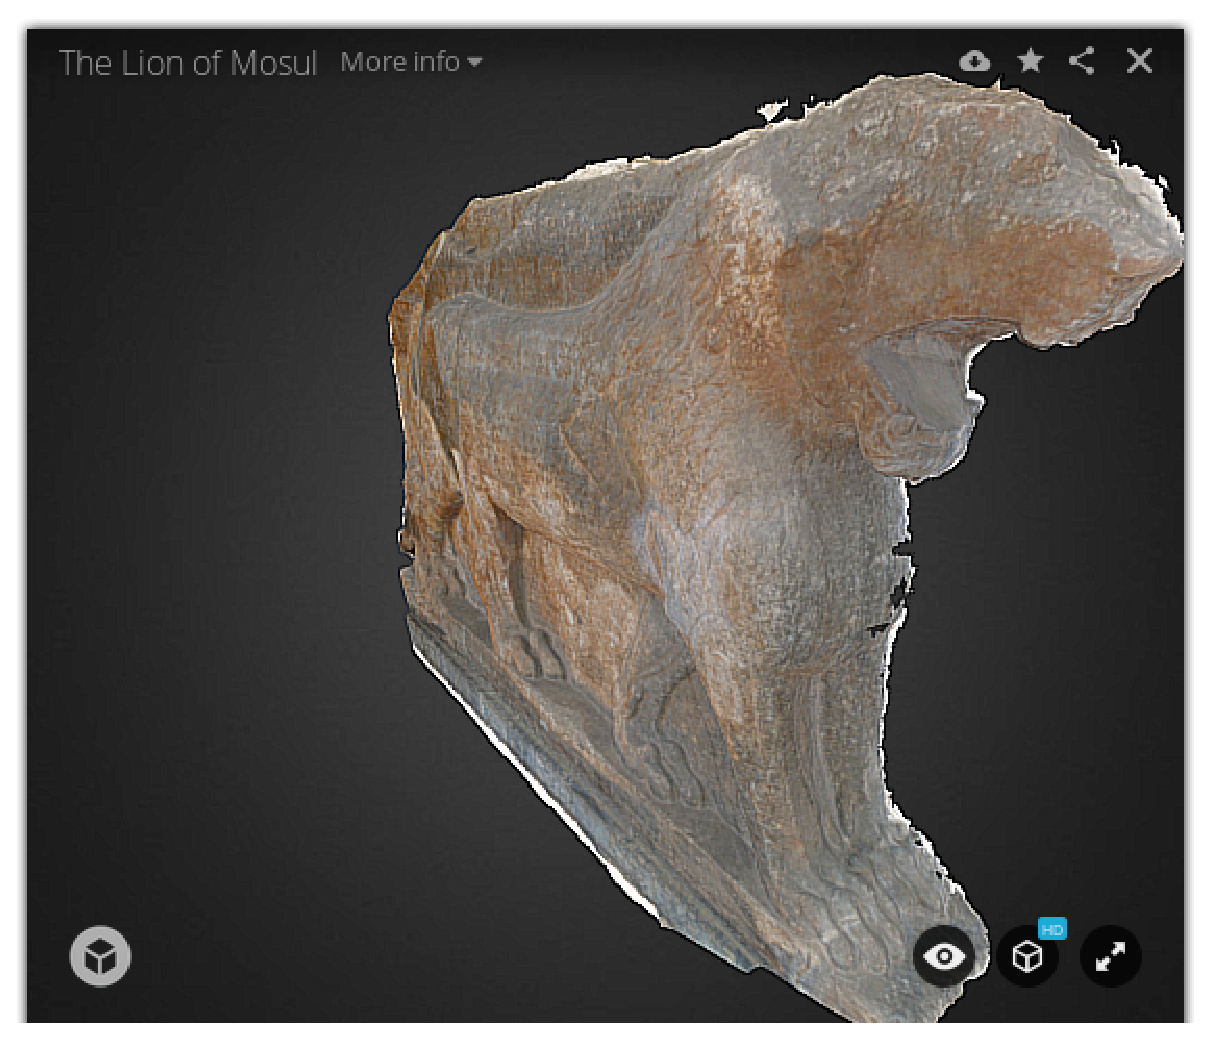
\includegraphics[scale=.18]{figuras/lion-mosul-2}}
%\end{figure}
\vspace{-.5 cm}
\begin{figure}[!htb]
\centering
\subfloat{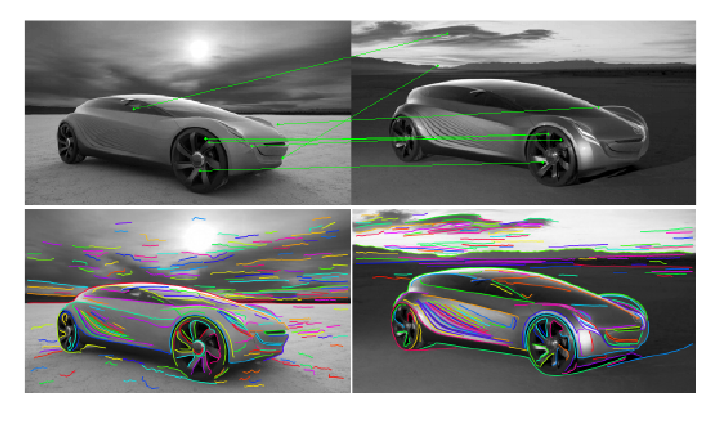
\includegraphics[scale=1]{figuras/carro}}
%\quad
%\subfloat{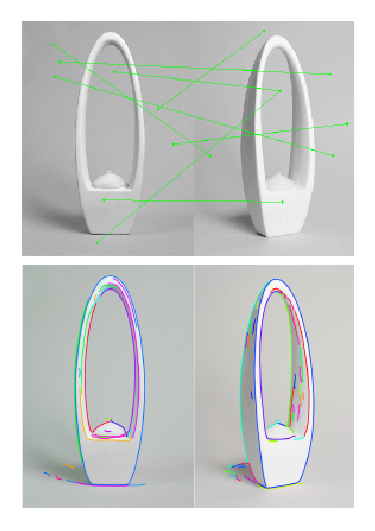
\includegraphics[scale=.47]{figuras/objeto-curvo}}
\end{figure}
}
%%
\frame{
\begin{figure}
\centering
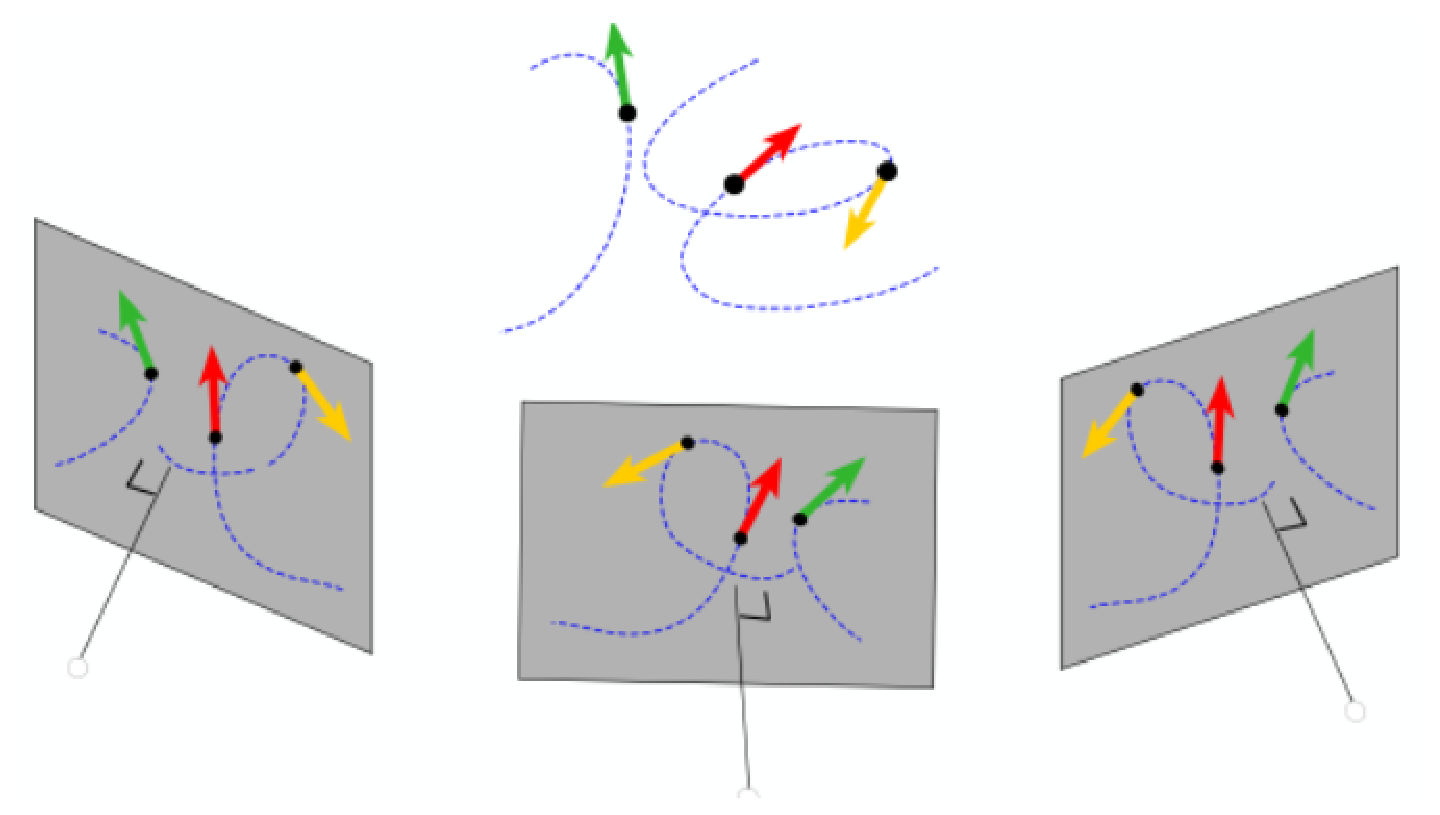
\includegraphics[scale=.33]{figuras/dife-tri}
\end{figure}
\begin{figure}
\centering
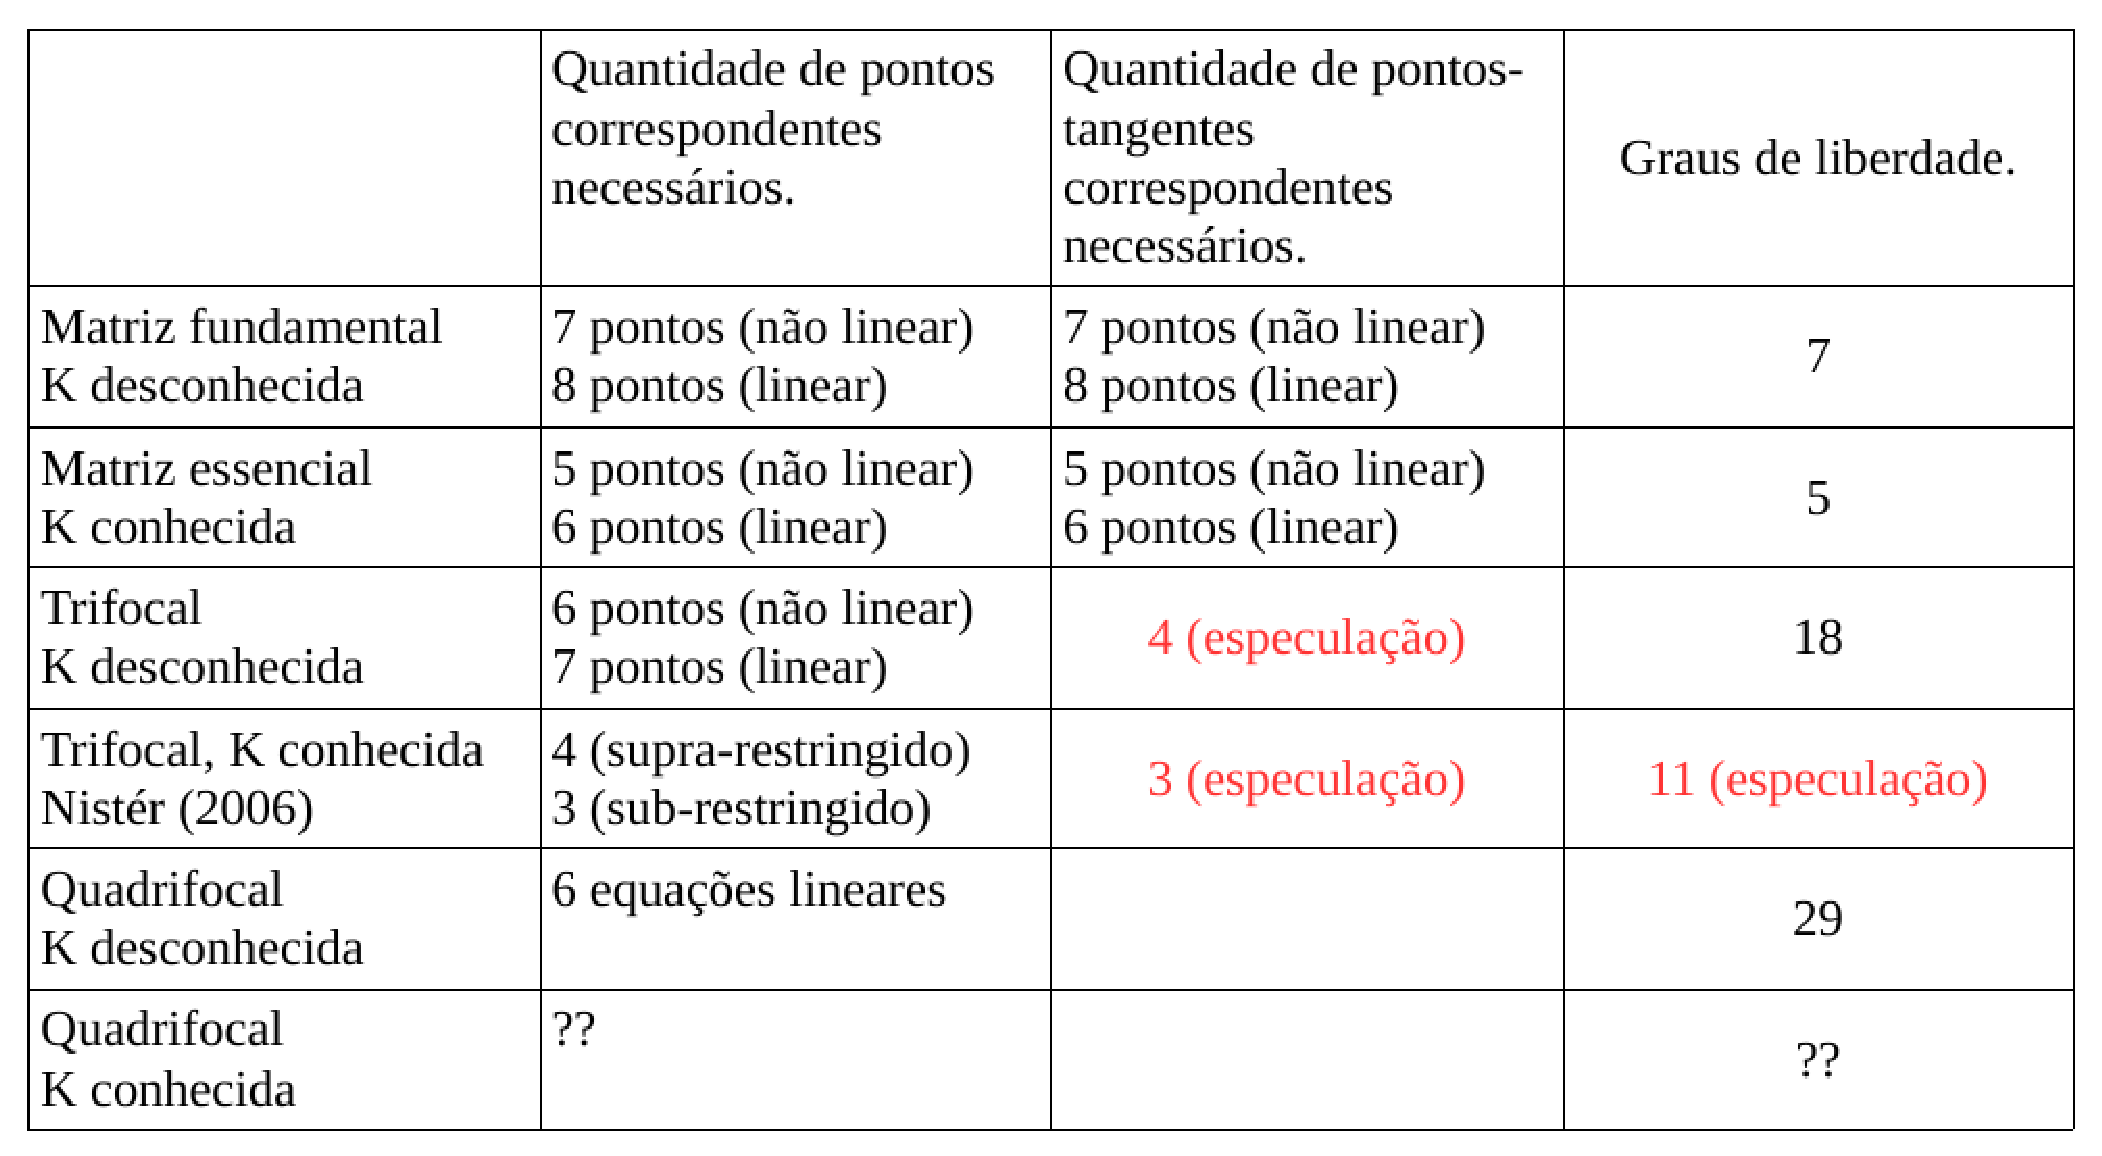
\includegraphics[scale=.18]{figuras/tab-dof}
\end{figure}
}
\section{Objetivos}
\frame{\frametitle{Principais objetivos}
\begin{enumerate}
\item Desenvolvimento de artigos recentes na busca por {\bf ferramentas matemáticas} que possam auxiliar nossa abordagem futura em {\bf reconstrução 3D} em termos de {\bf geometria diferencial trifocal}.
\\\quad\\
\item Levantamento dos {\bf benefícios} do uso da {\bf geometria trifocal} em correspondência de pontos de interesse em comparação geometria bifocal para cada par de câmeras num {\bf sistema multifocal}.

%\item Introduzir as ferramentas básicas de geometria projetiva necessárias ao estudo da reconstrução 3D usando geometria trifocal.
%\item Expor abordagem recente para reconstrução 3D de uma câmera utilizando o quatérnion de Hamilton e as bases de Gr\"obner.
%\item Levantamento teórico sobre geometria trifocal e verificação de suas vantagens em reconstrução 3D em detrimento da geometria epipolar bifocal.
%\item Detalhar matematicamente a geometria projetiva utilizada na abordagem mais eficiente para reconstrução de câmeras num sistema trifocal calibrado.
\end{enumerate}
}

%\section{Geometria de uma e duas câmeras}
%\frame{\frametitle{Retas, pontos, pontos ideais e reta no infinito}
%\begin{center}
%$a\,x+b\,y+c=0$\qquad $\lightrgb = (a,b,c)^\top \in \mathbb{R}^{3}$\\\quad\\
%
%$k\,(a,b,c)^\top$, tal que $k\neq 0$, representa a reta $k\,a\,x+k\,b\,y+k\,c=0$ que é a mesma reta $a\,x+b\,y+c=0$\\\quad\\
%
%{\it classe de equivalência}\qquad vetores {\it homogêneos}\\\quad\\
%  
%$\mathbb{R}^{3} - (0,0,0)^\top$ forma o {\it Espaço Projetivo} $\mathbb{P}^{2}$
%\end{center}
%\begin{center}
%$\x=(x,y,1)^\top$\qquad $a\,x+b\,y+c=0$
%\end{center}
%\begin{equation*}
%(x,y,1)^\top 
%\begin{pmatrix}
% a  \\ 
% b  \\ 
% c 
% \end{pmatrix} 
% = 0 \qquad 
% \text{ou} 
% \qquad \x ^\top\lightrgb = 0.
%\end{equation*}
%\begin{equation*}
%(k\,x,k\,y,k)^\top 
%\begin{pmatrix}
% a  \\ 
% b  \\ 
% c 
% \end{pmatrix} 
% = 0
% \qquad \Leftrightarrow \qquad
% (x,y,1)^\top
%\begin{pmatrix}
% a  \\ 
% b  \\ 
% c 
% \end{pmatrix} 
% = 0.
%\end{equation*}
%}
%%
%\frame{\frametitle{Retas, pontos, pontos ideais e reta no infinito}
%\begin{figure}[!htb]
%\centering
%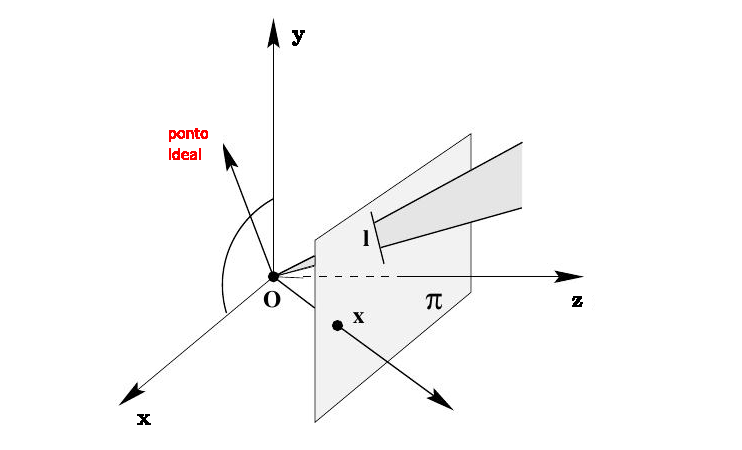
\includegraphics[scale=1]{figuras/espaco_P2}
%\end{figure}
%}
%%
%\frame{\frametitle{Retas, pontos, pontos ideais e reta no infinito}
%
%\begin{equation*}
%\lightrgb\cdot(\lightrgb\times\lightrgb')=\lightrgb'\cdot(\lightrgb\times\lightrgb')=0.
%\end{equation*}
%
%\begin{equation*}
%\lightrgb^\top(\lightrgb\times\lightrgb')=\lightrgb'^\top(\lightrgb\times\lightrgb')=0,
%\end{equation*}
%e sendo $\x$ o ponto de interseção entre as duas retas temos
%\begin{equation*}
%\lightrgb^\top\x=\lightrgb'^\top\x=0
%\end{equation*}
%onde, comparando
%\begin{equation*}
%\x=\lightrgb\times\lightrgb'
%\end{equation*}
%
%dualidade
%
%\begin{equation*}
%\lightrgb=\x\times\x'
%\end{equation*}\\
%}
%%
%\frame{\frametitle{Retas, pontos, pontos ideais e reta no infinito}
%\begin{equation*}
%\begin{array}{rcl}
%\lightrgb\times\lightrgb'&=&(a,b,c)^\top\times(a,b,c')^\top\\
%&=&(c'-c)\,(b,-a,0)^\top\\
%&=&(b,-a,0)^\top
%\end{array}
%\end{equation*}
%\begin{equation*}
%\left(\frac{b}{0},\frac{-a}{0}\right)^\top
%\end{equation*}
%\textit{pontos ideais} ou \textit{pontos no infinito} no plano projetivo.
%\begin{equation*}
%\lightrgb_\infty^\top \x=(0,0,1)
%\begin{pmatrix}
%x\\
%y\\
%0
%\end{pmatrix}
%=0,\qquad\text{\textit{reta no infinto}}
%\end{equation*} 
%$\lightrgb=(a,b,c)^\top$ interseção com  $\lightrgb_\infty=(0,0,1)^\top$,
%
%\begin{equation*}
%\lightrgb\times \lightrgb_\infty=(b,-a,0),
%\end{equation*}
%$(b,-a)$, é ortogonal ao vetor normal $(a,b)$
%}
%%
%\frame{\frametitle{Cônicas de pontos}
%\begin{equation*}
%a\,x^2+b\,x\,y+c\,y^2+d\,x+e\,y+f=0.
%\end{equation*}
%\begin{equation*}
%(x,y,1) 
% \begin{bmatrix}
%a & b/2 & d/2\\
%b/2 & c & e/2\\
%d/2 & e/2 & f
%\end{bmatrix}
% \begin{pmatrix}
%x\\
%y\\
%1
%\end{pmatrix}
% = 0.
%\end{equation*}
%multiplicando-se por um fator $x_3$ e definindo $x_1=x_3\,x$ e $x_2=x_3\,y$
%\begin{equation*}
%a\,x_1^2+b\,x_1\,x_2+c\,x_2^2+d\,x_1\,x_3+e\,x_2\,x_3+f\,x_3^2=0.
%\end{equation*}
%\begin{equation*}
%(x_1,x_2,x_3) 
% \begin{bmatrix}
%  a & b/2 & d/2\\
%  b/2 & c & e/2\\
%  d/2 & e/2 & f
%  \end{bmatrix}
% \begin{pmatrix}
%  x_1\\
%  x_2\\
%  x_3
%  \end{pmatrix}
% = 0
% \qquad \text{ou} \qquad
% \x^\top C\,\x = 0.
%\end{equation*}
%\begin{equation*}
%C =  \begin{bmatrix}
%      a & b/2 & d/2\\
%      b/2 & c & e/2\\
%      d/2 & e/2 & f
%      \end{bmatrix}.
%\end{equation*}
%}
%%
%\frame{\frametitle{Cônicas de retas e cônicas degeneradas}
%Cônica dual denotada por $C^*$
%\begin{figure}[!htb]
%\centering
%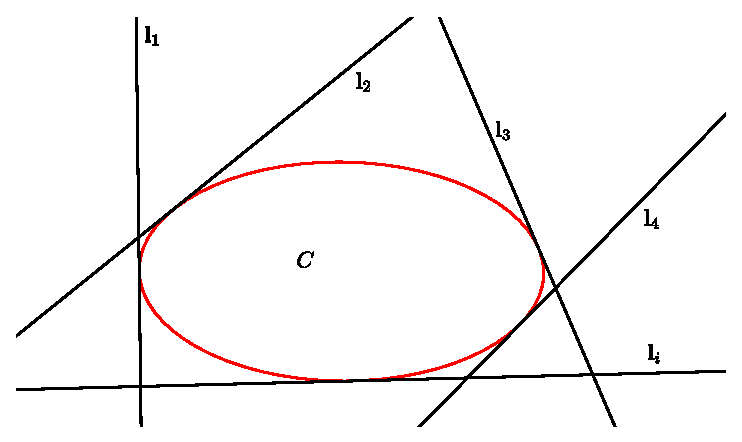
\includegraphics[scale=.7]{figuras/conica-envelope}
%\end{figure}
%
%\begin{equation*}
%C=\lightrgb\,{\bf m}^\top+{\bf m}\,\lightrgb^\top
%\end{equation*}
%}
%%
%\frame{\frametitle{A relação polo-polar  e pontos conjugados}
%\begin{equation*}
%\lightrgb=C\,\x.
%\end{equation*}
%\begin{figure}[!htb]
%\centering
%\subfloat{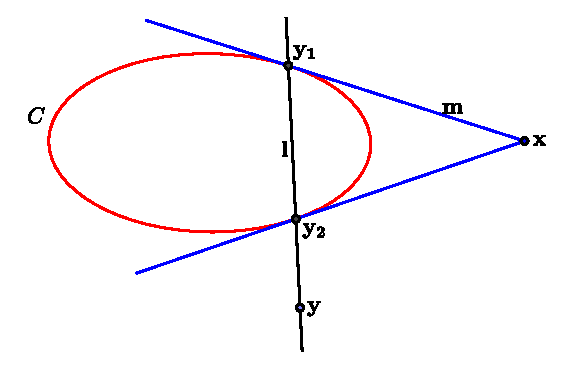
\includegraphics[scale=.6]{figuras/polo-polar}}
%\quad
%\subfloat{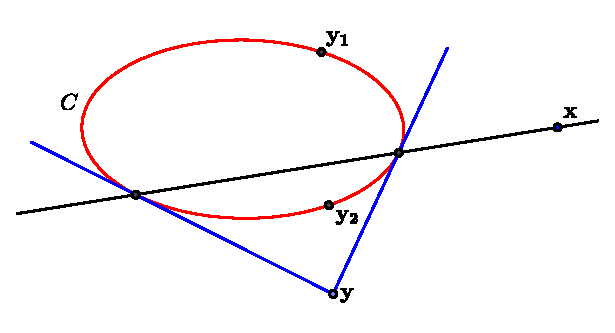
\includegraphics[scale=.6]{figuras/polo-polar-simetria}}
%\end{figure}
%}
%%
%\frame{\frametitle{Transformações projetivas em $\mathbb{P}^2$}
%$h:\mathbb{P}^2\rightarrow\mathbb{P}^2$ é uma transformação projetiva se, e somente se, existe uma matriz $H_{3\times3}$ onde para cada ponto $\x\in\mathbb{P}^2$ temos que $h(\x)=H\,\x$
%\begin{equation*}
%\x'=H\,\x,
%\end{equation*}
%os pontos $\x\leftrightarrow\x'$ são chamados {\it pontos correspondentes}
%
%\begin{equation*}
%\begin{pmatrix}
%x'\\
%y'
%\end{pmatrix}
%=
%R
%\begin{pmatrix}
%x\\
%y
%\end{pmatrix}+
%\begin{pmatrix}
%t_x\\
%t_y
%\end{pmatrix}
%\end{equation*}\\\quad\\
%\begin{equation*}
%\begin{pmatrix}
%x'\\
%y'\\
%1
%\end{pmatrix}
%=
%\begin{bmatrix}
%cos\,\theta&-sen\,\theta&t_x\\
%sen\,\theta&cos\,\theta&t_y\\
%0&0&1
%\end{bmatrix}
%\begin{pmatrix}
%x\\
%y\\
%1
%\end{pmatrix}
%\end{equation*}
%}
%%
%\frame{\frametitle{Subgrupo de transformações projetivas}
%\begin{figure}[!htb]
%\centering
%\subfloat{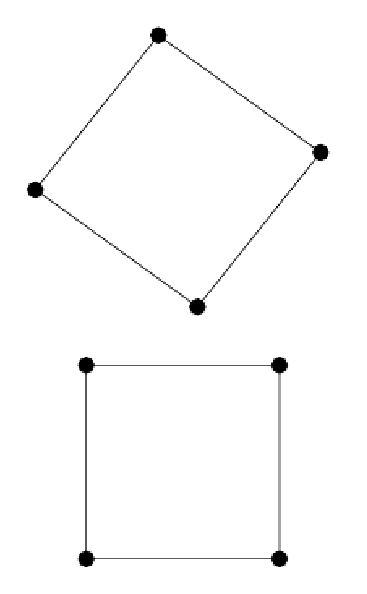
\includegraphics[scale=.42]{figuras/trans-euclidiana-2D}}
%\qquad
%\subfloat{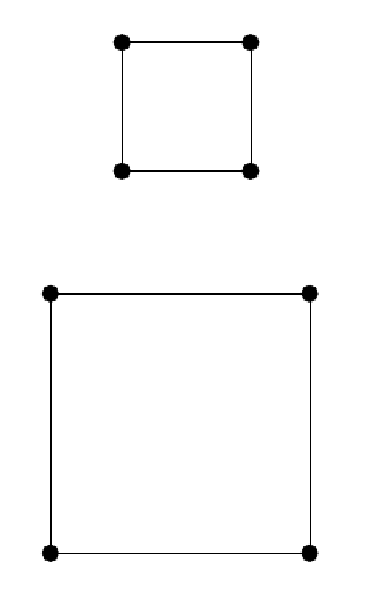
\includegraphics[scale=.42]{figuras/trans-similaridade-2D}}
%\qquad
%\subfloat{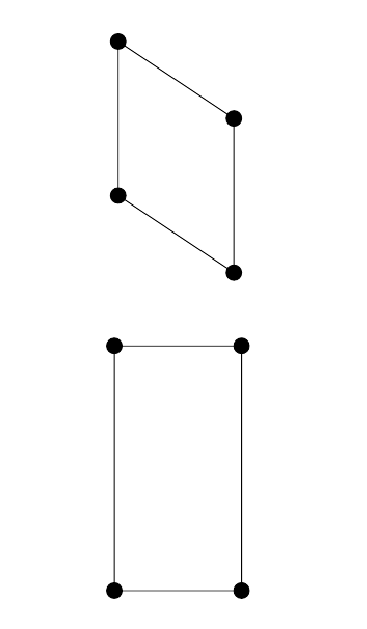
\includegraphics[scale=.42]{figuras/trans-afinidade-2D}}
%\qquad
%\subfloat{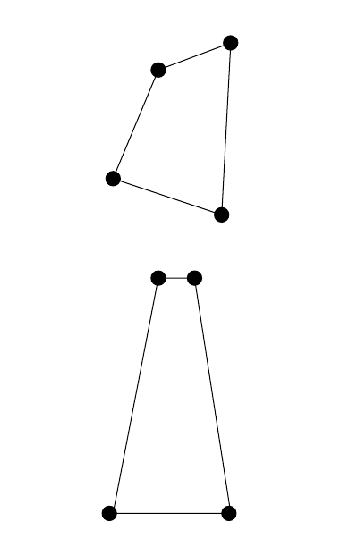
\includegraphics[scale=.42]{figuras/trans-projetividade-2D}}
%\end{figure}
%}
%%
%\frame{\frametitle{A geometria projetiva de uma dimensão}
%\begin{equation*}
%\overline{\x}=
%\begin{pmatrix}
%x_1\\
%x_2
%\end{pmatrix}
%\qquad\text{e}\qquad
%\overline{\x}'=H\,\overline{\x}
%\end{equation*}
%\begin{figure}[!htb]
%\centering
%\subfloat{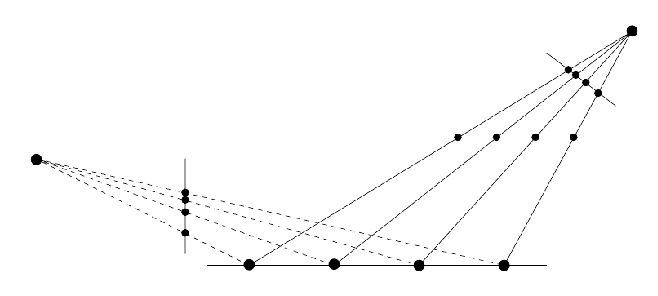
\includegraphics[scale=.7]{figuras/geometria-P1}}
%\quad
%\subfloat{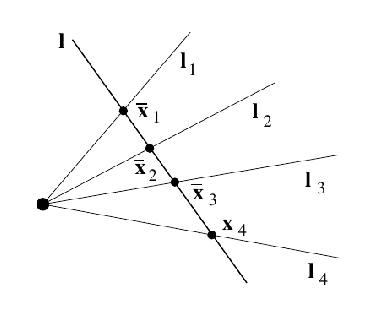
\includegraphics[scale=.7]{figuras/razao-cruzada-retas}}
%\end{figure}
%\begin{equation*}
%\text{cross}(\overline{\x}_1,\overline{\x}_2,\overline{\x}_3,\overline{\x}_4)=\frac{|\overline{\x}_1\,\overline{\x}_2||\overline{\x}_3\,\overline{\x}_4|}{|\overline{\x}_1\,\overline{\x}_3||\overline{\x}_2\,\overline{\x}_4|}
%\end{equation*}
%}
%
%\frame{\frametitle{A cônica absoluta}
%A cônica absoluta é uma cônica (ponto no infinito) denotada por $\Omega_\infty$ e está contida no plano no infinito $\bpi_\infty$.
%\begin{equation*}
%{\bf X}^\top\Omega_\infty{\bf X}=0
%\end{equation*}
%}
%


%\frame{\frametitle{A câmera $P$}
%\begin{minipage}{.6\textwidth}
%\begin{center}
%$
%\x=P\,\X
%$
%\end{center}
%\begin{equation*}
%P = K \, [I|{\bf 0}]
%\begin{bmatrix}
%R&{\bf t}\\
%\,\,{\bf 0}^\top &1
%\end{bmatrix}
%= K\,[R|{\bf t}]
%\end{equation*}
%\begin{center}
%$
%\x=K\,[R|{\bf t}]\,\X
%$
%\end{center}
%\end{minipage}
%\begin{minipage}{.3\textwidth}
%\begin{equation*}
%K = \begin{bmatrix}
%\alpha_x & \sigma & p_x\\
%0 &\alpha_y &  p_y\\
%0 & 0 &  1
%\end{bmatrix}
%\end{equation*}
%\end{minipage}
%\begin{figure}[!htb]
%\centering
%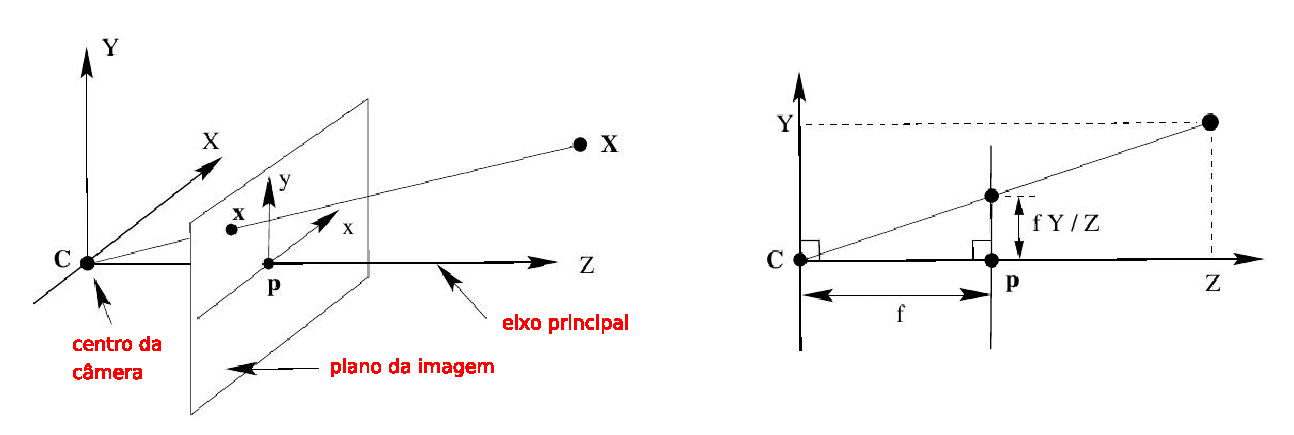
\includegraphics[scale=.58]{figuras/modelo_camera}
%\end{figure}
%}
%


%\frame{\frametitle{Resumo dos parâmetros da câmera}
%\begin{table}
%\begin{center}
%\begin{tabular}{c l} 
%\textbf{Variáveis Livres} & \textbf{Descrição}\\
%3	 & rotação \\
%3	 & translação \\
%2	 & mudança de escala em $x,y$\\
%1	 & distância focal\\
%2	 & ponto principal\\
%1	 & ângulo entre os eixos \\
%6  & total extrinsecos\\
%6  & total intrinsecos\\
%12 & total\\
%11 & total único (distância focal para fixar escala)
%\end{tabular}
%\end{center}
%\end{table}
%}
%%
%\frame{\frametitle{Geometria epipolar}
%\begin{figure}[!htb]
%\centering
%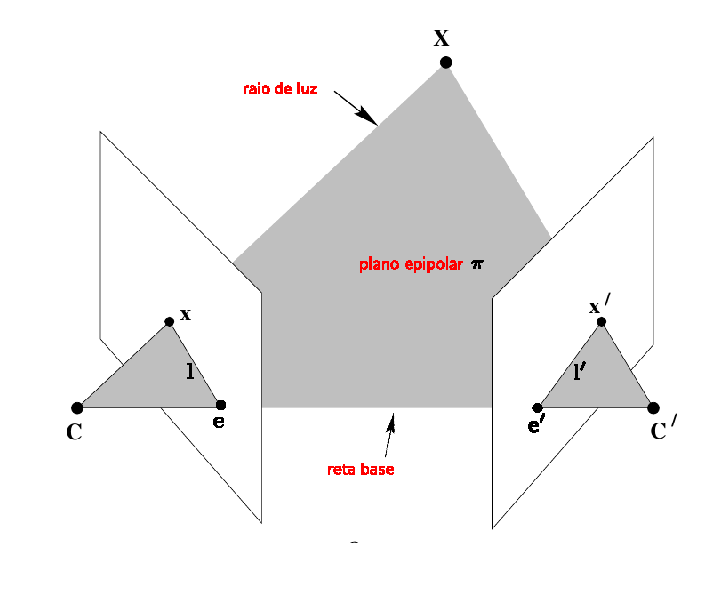
\includegraphics[scale=.9]{figuras/geometria-epipolar}
%\end{figure}
%}
%%
%\frame{\frametitle{A matriz fundamental}
%\begin{figure}[!htb]
%\centering
%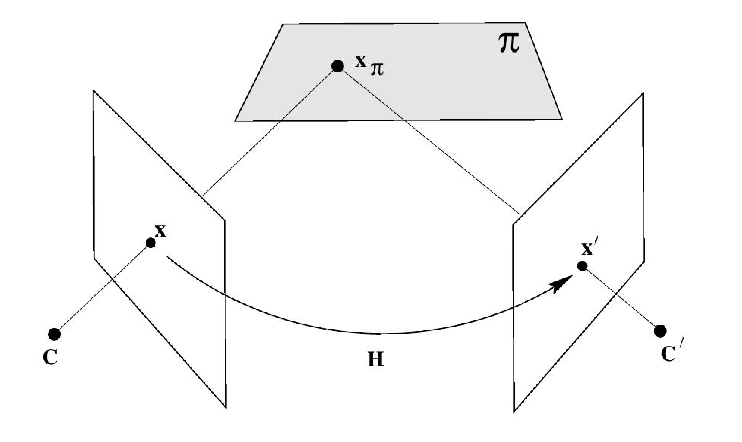
\includegraphics[scale=.7]{figuras/homografia}
%\end{figure}
%\begin{minipage}{.5\textwidth}
%\begin{equation*}
%\x'_i= H_{\bpi} \,\x_i
%\end{equation*}
%\end{minipage}
%\begin{minipage}{.4\textwidth}
%\begin{equation*}
%\begin{array}{rcl}
%\lightrgb'&=&\e'\times\x'\\
%\end{array}
%\end{equation*}
%\end{minipage}
%\begin{equation*}
%\begin{array}{rcl}
%\lightrgb'&=&[\e']_\times\x'\\
%&=&[\e']_\times H_{\bpi} \,\x\\
%&=&F\,\x,
%\end{array}
%\end{equation*}
%}
%%
%\frame{\frametitle{Condição de correspondência e a matriz essencial}
%\begin{equation*}
%\begin{array}{rcl}
%\lightrgb'&=&F\,\x\\
%\x'^\top\lightrgb'&=&\x'^\top F\,\x\\
%0&=&\x'^\top F\,\x.
%\end{array}
%\end{equation*}
%A relação acima é denominda {\it condição de correspondência}.
%\begin{center}
%$P=K\,[R|{\bf t}]$ $\longrightarrow$ $P=[R|{\bf t}]$
%\end{center}
%chamada {\it câmera normalizada}. 
%\begin{equation*}
%\hat{\x}=P\,{\bf X}=[R|{\bf t}]\,\X
%\end{equation*}
%onde o ponto $\hat{\x}$ é dito estar em {\it coordenadas  normalizadas}.
%\begin{equation*}
%P=[I|{\bf 0}]\qquad\text{e}\qquad P'=[R|{\bf t}]
%\end{equation*}
%\begin{equation*}
%E=[{\bf t}]_\times R
%\end{equation*}
%}
%
\frame{
\begin{center}
\textcolor{blue}{{\large Determinação de uma câmera\\\quad\\
Kuang e {\AA}str{\"o}m [2013]}}
\end{center}
\begin{figure}
\centering
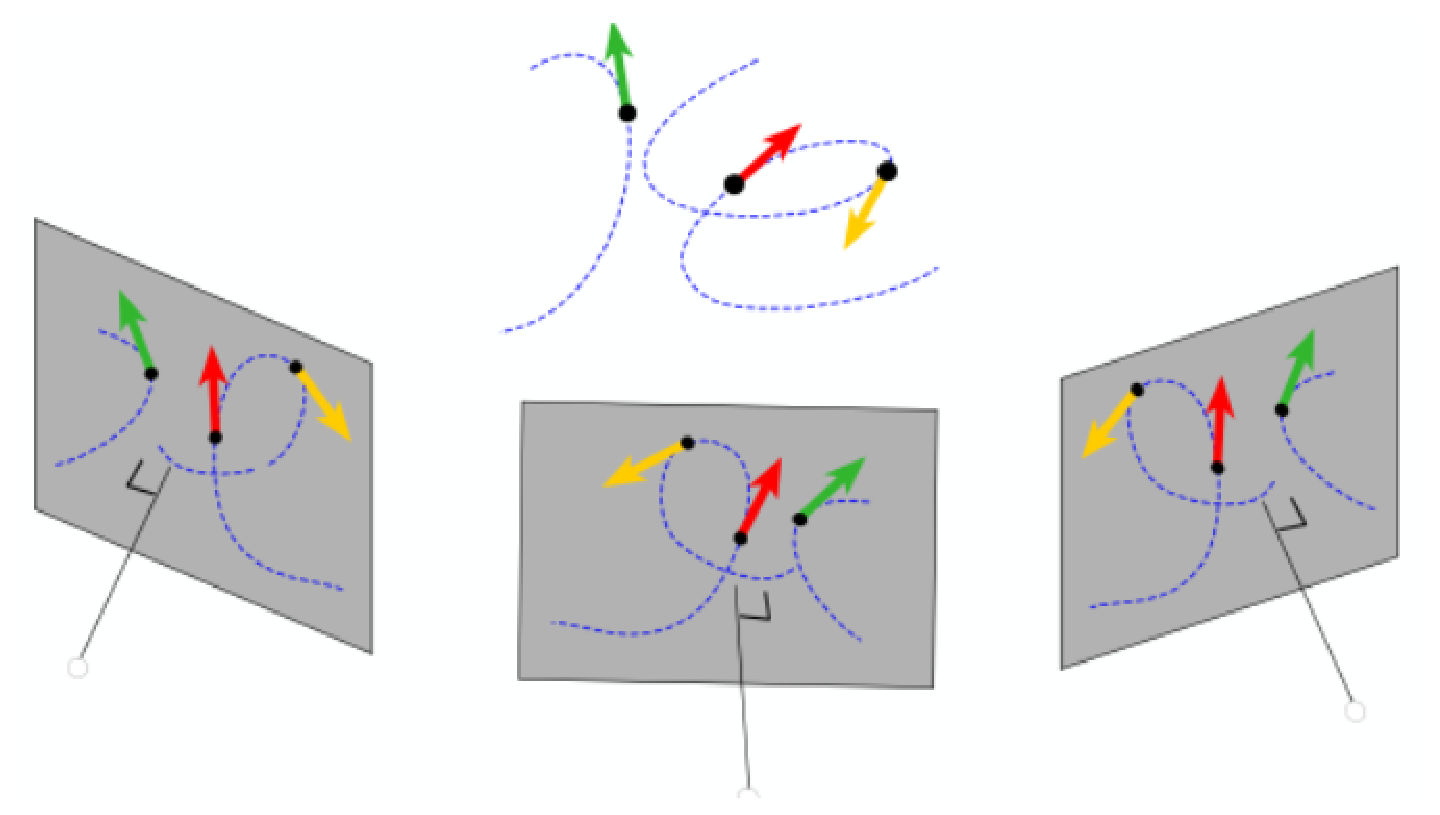
\includegraphics[scale=.45]{figuras/dife-tri}
\end{figure}
}


\section{Kuang e {\AA}str{\"o}m [2013]}
\frame{\frametitle{Kuang e {\AA}str{\"o}m [2013]}
\begin{minipage}{.4\textwidth}
\begin{equation*}
\lambda\,\x=P\,\X
\end{equation*}
\begin{equation*}
P=K\,[R|{\bf t}]
\end{equation*}
\end{minipage}
\begin{minipage}{.5\textwidth}
\begin{equation*}
K=
\begin{bmatrix}
1&0&0\\
0&1&0\\
0&0&w
\end{bmatrix}\quad\text{onde}\quad w=\frac{1}{f}
\end{equation*}
\end{minipage}
\begin{figure}[!htb]
\centering
\includegraphics[scale=.8]{figuras/camera-astrom}
\end{figure}
}
\frame{\frametitle{}
\begin{figure}[!htb]
\centering
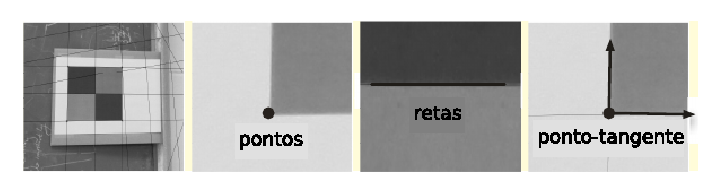
\includegraphics[scale=.8]{figuras/astrom-objetos-geo}
\end{figure}
usando pontos
\begin{equation*}
[\x]_\times P\,\X={\bf 0}
\end{equation*}
retas
\begin{equation*}
\begin{array}{rcll}
\lightrgb^\top P\,\X&=&0&\text{se}\,\,\,k=0\\
\lightrgb^\top P({\bf X}+k\,{\bf D})&=&0&\text{se}\,\,\,k\neq0
\end{array}
\end{equation*}
pontos-tangentes
\begin{equation*}
\lightrgb^\top P\,{\bf D}=0.
\end{equation*}
\begin{center}
\begin{tabular}{|c|c|c|c|}
\hline 
{\bf ponto} & {\bf reta} & {\bf ponto com 1 tangente} & {\bf ponto com 2 tangentes} \\ 
\hline 
2 & 2 & 3 & 4 \\ 
\hline 
\end{tabular} 
\end{center}
\begin{center}
casos úteis: 2P1T e 1T2T
\end{center}
}
%
\frame{\frametitle{Parametrização de $P$ e sistemas de polinômios}
\begin{equation*}
R=
\begin{bmatrix}
a^2+b^2-c^2-d^2&2bc-2ad&2ac+2bd\\
2ad+2bc&a^2-b^2+c^2-d^2&2cd-2ab\\
2bd-2ac&2ab+2cd&a^2-b^2-c^2+d^2
\end{bmatrix}
\end{equation*}\\\quad\\
\begin{equation*}
P=K\,[R|{\bf t}]
\end{equation*}\\\quad\\
\begin{equation*}
\begin{bmatrix}
a^2+b^2-c^2-d^2&2bc-2ad&2ac+2bd&t_x\\
2ad+2bc&a^2-b^2+c^2-d^2&2cd-2ab&t_y\\
w\,(2bd-2ac)&w\,(2ab+2cd)&w\,(a^2-b^2-c^2+d^2)&w\,t_z
\end{bmatrix}
\end{equation*}\\\quad\\
\begin{center}
$\{b,c,d,w\}$
\end{center}
}
%
\frame{\frametitle{Contribuições}
\begin{enumerate}
\item Quatérnions para parametrizar a rotação.
\\\quad\\
\item Resolve uma parte do problema de reconstrução das três câmeras.
\\\quad\\
\item Utilização de correspondência entre pontos-tangentes.
\\\quad\\
\item Geometria algébrica na solução de sistemas de equações polinomiais com várias variáveis. 
\end{enumerate}
}
%
\frame{
\begin{center}
\textcolor{blue}{{\large Geometria trifocal}}
\end{center}
\begin{figure}
\centering
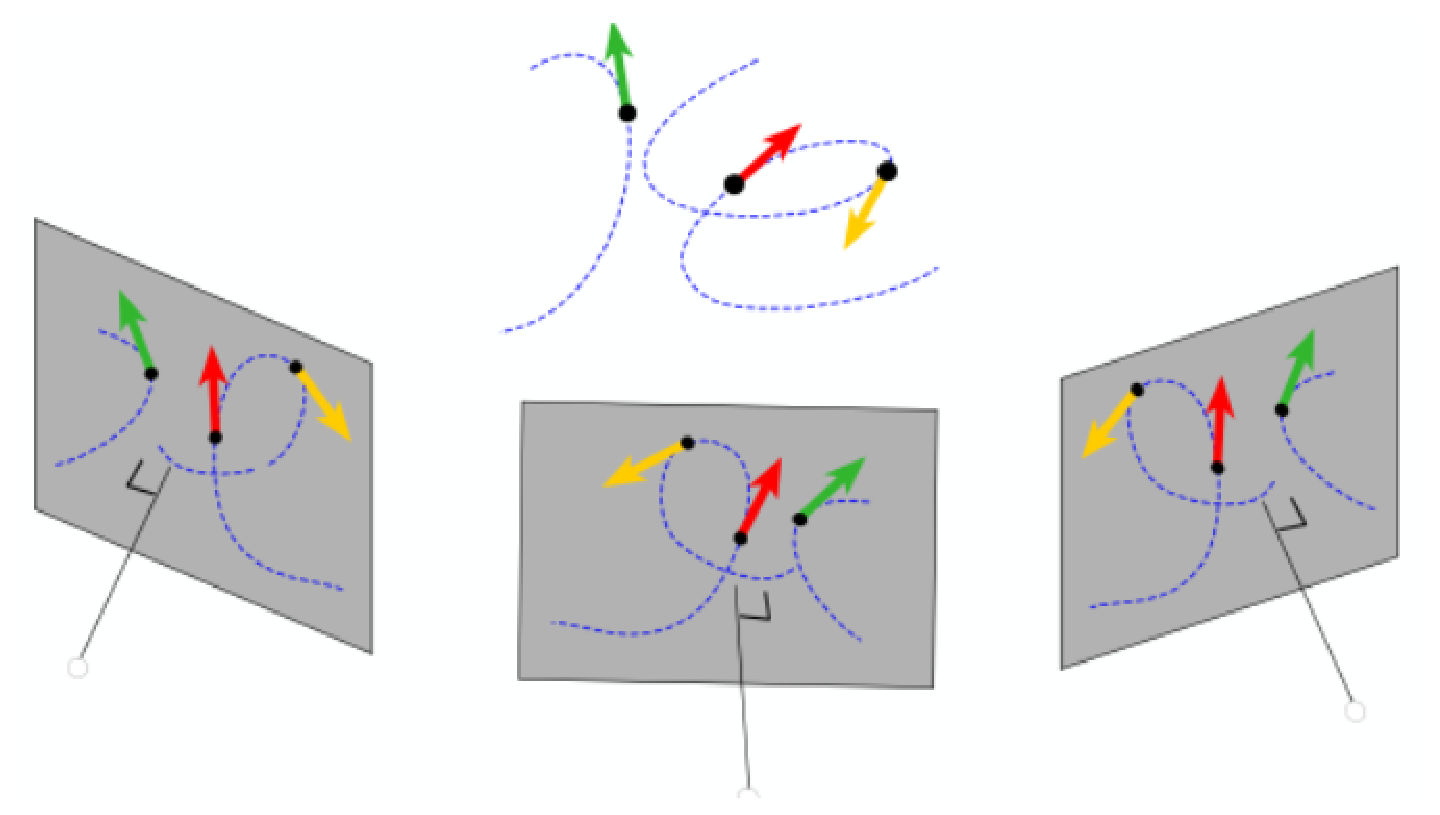
\includegraphics[scale=.45]{figuras/dife-tri}
\end{figure}
}
\section{Geometria trifocal}
\frame{\frametitle{Geometria trifocal e transferência epipolar}
\begin{figure}
\centering
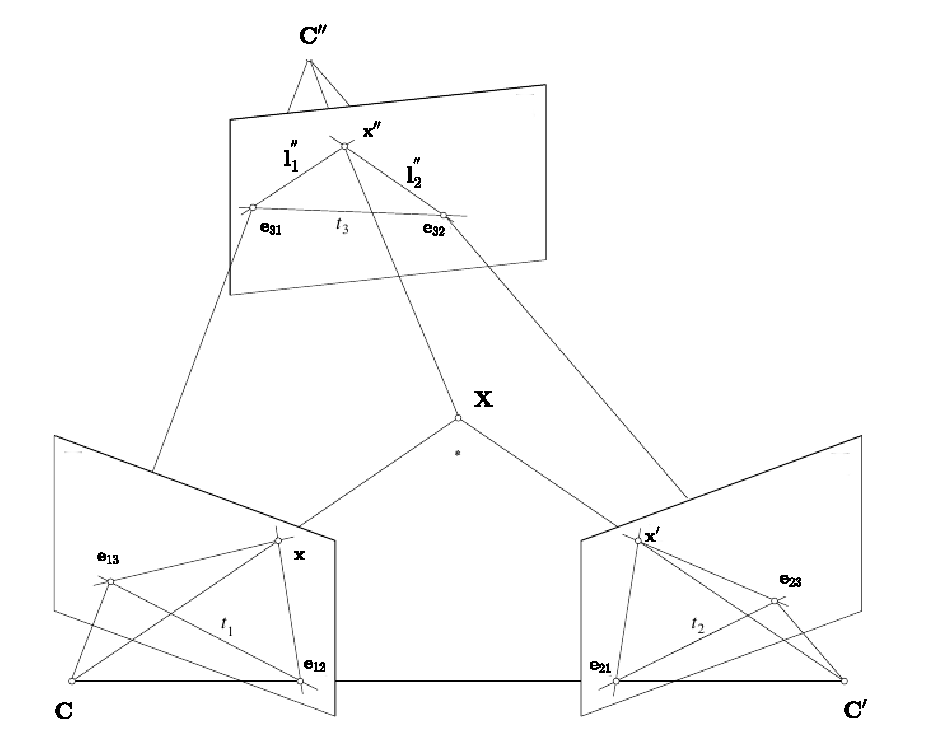
\includegraphics[scale=.67]{figuras/trifocal-frente-frente}
\end{figure}
%\begin{equation*}
%\begin{array}{rcl}
%\x''&=&\lightrgb''_1\times\lightrgb''_2\\
%\x''&=&F_{31}\x\times F_{32}\x'.
%\end{array}
%\end{equation*}
}
%
\frame{\frametitle{O tensor trifocal}
\begin{figure}[!htb]
\centering
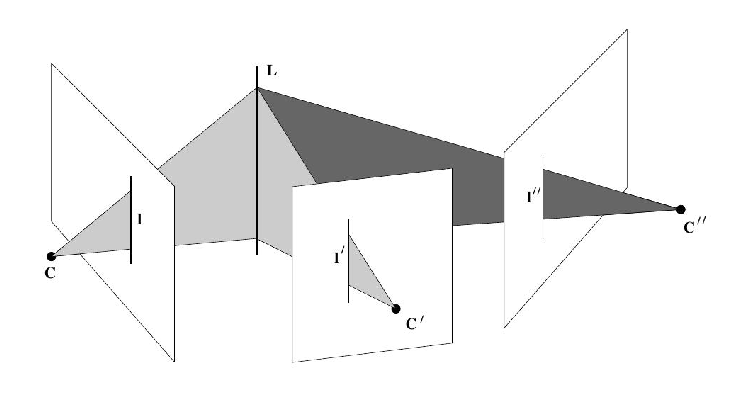
\includegraphics[scale=.6]{figuras/abord-geo-tri}
\end{figure}
\begin{center}
$P=[I|{\bf 0}]$\quad $P'=[A|{\bf a}_4]$\quad $P''=[B|{\bf b}_4]$
\end{center}
\vspace{.4 cm}
\begin{equation*}
\begin{array}{rcl}
\pi&=&P^\top\lightrgb\\
\pi&=&
\begin{pmatrix}
\lightrgb\\
0
\end{pmatrix}
\end{array},\qquad
\begin{array}{rcl}
\pi'&=&P'^\top\lightrgb'\\
\pi'&=&
\begin{pmatrix}
A^\top\lightrgb'\\
{\bf a}^\top_4\lightrgb'
\end{pmatrix}
\end{array}\quad\text{e}\quad
\begin{array}{rcl}
\pi''&=&P''^\top\lightrgb''\\
\pi''&=&
\begin{pmatrix}
B^\top\lightrgb''\\
{\bf b}^\top_4\lightrgb''
\end{pmatrix}
\end{array}.
\end{equation*}
\vspace{.4 cm}
\begin{equation*}
M=
\begin{bmatrix}
\lightrgb&A^\top\lightrgb'&B^\top\lightrgb''\\
0&{\bf a}^\top_4\lightrgb'&
{\bf b}^\top_4\lightrgb''
\end{bmatrix}
\end{equation*}
}
%
\frame{\frametitle{}
\begin{center}
${\bf X}\in{\bf L}$\qquad ${\bf X}=\lambda_1{\bf X}_1+\lambda_2{\bf X}_2$\\
\vspace{.3 cm}
$\bpi^\top{\bf X}=0$\qquad $\bpi'^\top{\bf X}=0$\qquad $\bpi''^\top{\bf X}=0$\qquad\qquad $M^\top{\bf X}={\bf 0}$
\end{center}
\vspace{.3 cm}
\begin{equation*}
\begin{pmatrix}
\lightrgb\\
0
\end{pmatrix}
=
\alpha
\begin{pmatrix}
A^\top\lightrgb'\\
{\bf a}^\top_4\lightrgb'
\end{pmatrix}
+\beta
\begin{pmatrix}
B^\top\lightrgb''\\
{\bf b}^\top_4\lightrgb''
\end{pmatrix}.
\end{equation*}
\vspace{.2 cm}
\begin{equation*}
\alpha=k\,{\bf b}^\top_4\lightrgb''\quad\text{e}\quad\beta=-k\,{\bf a}^\top_4\lightrgb'\quad\Rightarrow\quad0=\alpha\,{\bf a}^\top_4\lightrgb'+\beta\,{\bf b}^\top_4\lightrgb''.
\end{equation*}
\vspace{.2 cm}
\begin{equation*}
\begin{array}{rcl}
\lightrgb&=&\alpha\,A^\top\lightrgb'+\beta\,B^\top\lightrgb''\\
\lightrgb&=&({\bf b}^\top_4\lightrgb'')A^\top\lightrgb'-({\bf a}^\top_4\lightrgb')B^\top\lightrgb''\\
\lightrgb&=&(\lightrgb''^\top{\bf b}_4)A^\top\lightrgb'-(\lightrgb'^\top{\bf a}_4)B^\top\lightrgb''.
\end{array}
\end{equation*}
\begin{equation*}
\begin{array}{rcl}
l_i&=&\lightrgb''^\top({\bf b}_4{\bf a}^\top_i)\lightrgb'-\lightrgb'^\top({\bf a}_4{\bf b}_i^\top)\lightrgb''\\
l_i&=&\lightrgb'^\top({\bf a}_i{\bf b}^\top_4)\lightrgb''-\lightrgb'^\top({\bf a}_4{\bf b}_i^\top)\lightrgb''\\
l_i&=&\lightrgb'^\top({\bf a}_i{\bf b}^\top_4-{\bf a}_4{\bf b}_i^\top)\lightrgb''\\
l_i&=&\lightrgb'^\top \mbox{T}_i\lightrgb'',
\end{array}
\end{equation*}
onde definimos $\mbox{T}_i={\bf a}_i{\bf b}^\top_4-{\bf a}_4{\bf b}_i^\top$
}
%
%\frame{\frametitle{Relações de incidência}
%\begin{minipage}{.4\textwidth}
%\begin{equation*}
%\lightrgb=
%\begin{pmatrix}
%\lightrgb'^\top \mbox{T}_1\lightrgb''\\
%\lightrgb'^\top \mbox{T}_2\lightrgb''\\
%\lightrgb'^\top \mbox{T}_3\lightrgb''
%\end{pmatrix}
%\end{equation*}
%\begin{equation*}
%\lightrgb'^\top(\sum_{i=1}^3 x^i\mbox{T}_i)\lightrgb''=0
%\end{equation*}
%\end{minipage}
%\begin{minipage}{.5\textwidth}
%\begin{equation*}
%\lightrgb'^\top(\sum_{i=1}^3 x^i\mbox{T}_i)[\x'']_\times={\bf 0}^\top
%\end{equation*}
%\begin{equation*}
%[\x']_\times(\sum_{i=1}^3 x^i\mbox{T}_i)[\x'']_\times=0_{3\times3}.
%\end{equation*}
%\end{minipage}
%\begin{figure}[!htb]
%\centering
%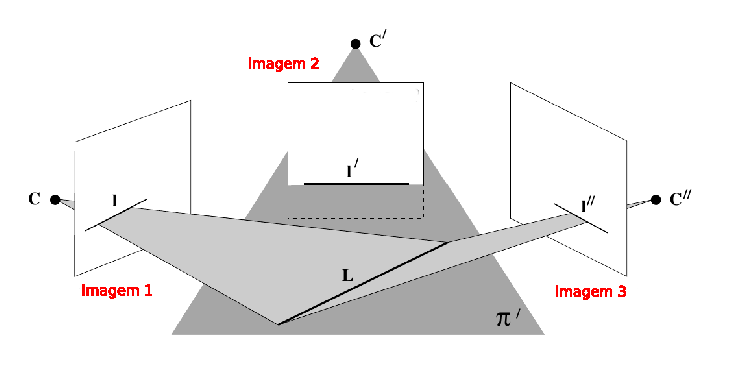
\includegraphics[scale=.85]{figuras/transfer-retas}
%\end{figure}
%}
%
\frame{\frametitle{Correspondência entre pontos usando o tensor trifocal}
\begin{minipage}{.3\textwidth}
\begin{equation*}
\lightrgb=
\begin{pmatrix}
\lightrgb'^\top \mbox{T}_1\lightrgb''\\
\lightrgb'^\top \mbox{T}_2\lightrgb''\\
\lightrgb'^\top \mbox{T}_3\lightrgb''
\end{pmatrix}
\end{equation*}
\end{minipage}
\begin{minipage}{.3\textwidth}
\begin{equation*}
\lightrgb'^\top(\sum_{i=1}^3 x^i\mbox{T}_i)\lightrgb''=0
\end{equation*}
\end{minipage}
\begin{minipage}{.3\textwidth}
\begin{equation*}
\x''=(\sum_{i=1}^3 x^i\mbox{T}_i^\top)\,\lightrgb'
\end{equation*}
\end{minipage}
\begin{figure}[!htb]
\centering
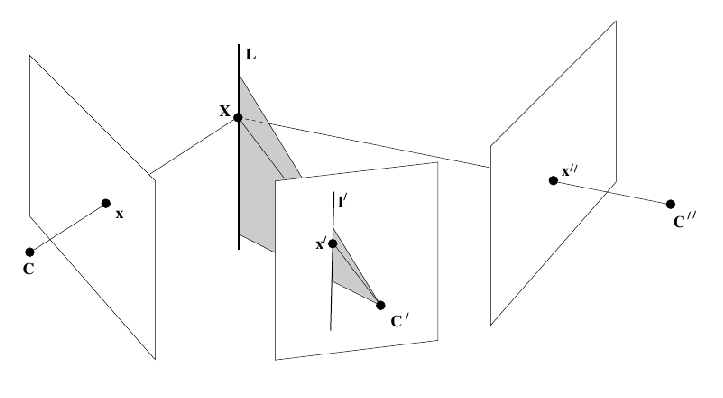
\includegraphics[scale=1]{figuras/X-plano-trifocal}
\end{figure}
}
%
\frame{\frametitle{Correspondência entre retas usando o tensor trifocal}
\begin{minipage}{.4\textwidth}
\begin{equation*}
\lightrgb=
\begin{pmatrix}
\lightrgb'^\top \mbox{T}_1\lightrgb''\\
\lightrgb'^\top \mbox{T}_2\lightrgb''\\
\lightrgb'^\top \mbox{T}_3\lightrgb''
\end{pmatrix}
\end{equation*}
\end{minipage}
\begin{minipage}{.5\textwidth}
\begin{equation*}
\lightrgb\times
\begin{pmatrix}
\lightrgb'^\top \mbox{T}_1\lightrgb''\\
\lightrgb'^\top \mbox{T}_2\lightrgb''\\
\lightrgb'^\top \mbox{T}_3\lightrgb''
\end{pmatrix}={\bf 0}
\end{equation*}
\end{minipage}
\begin{figure}[!htb]
\centering
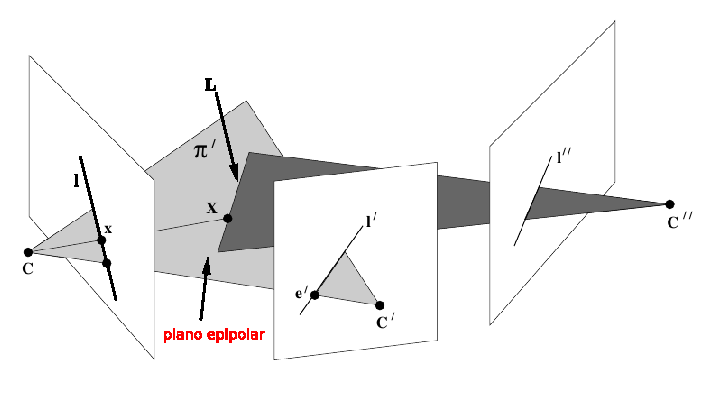
\includegraphics[scale=1]{figuras/plano-epipolar-tri}
\end{figure}
}
%
\frame{\frametitle{Contribuições}
\begin{enumerate}
\item Redução de quatro para apenas um caso de degeneração.
\\\quad\\
\item Correspondência direta entre retas.
\\\quad\\
\item Reconstrução de câmeras paralelas.
\\\quad\\
\item Melhor modelagem para correspondência entre curvas usando geometria diferencial. 
\end{enumerate}
}
%
\frame{
\begin{center}
\textcolor{blue}{{\large Geometria trifocal calibrada\\\quad\\
Nistér e  Schaffalitzky [2006]}}
\end{center}
\begin{figure}
\centering
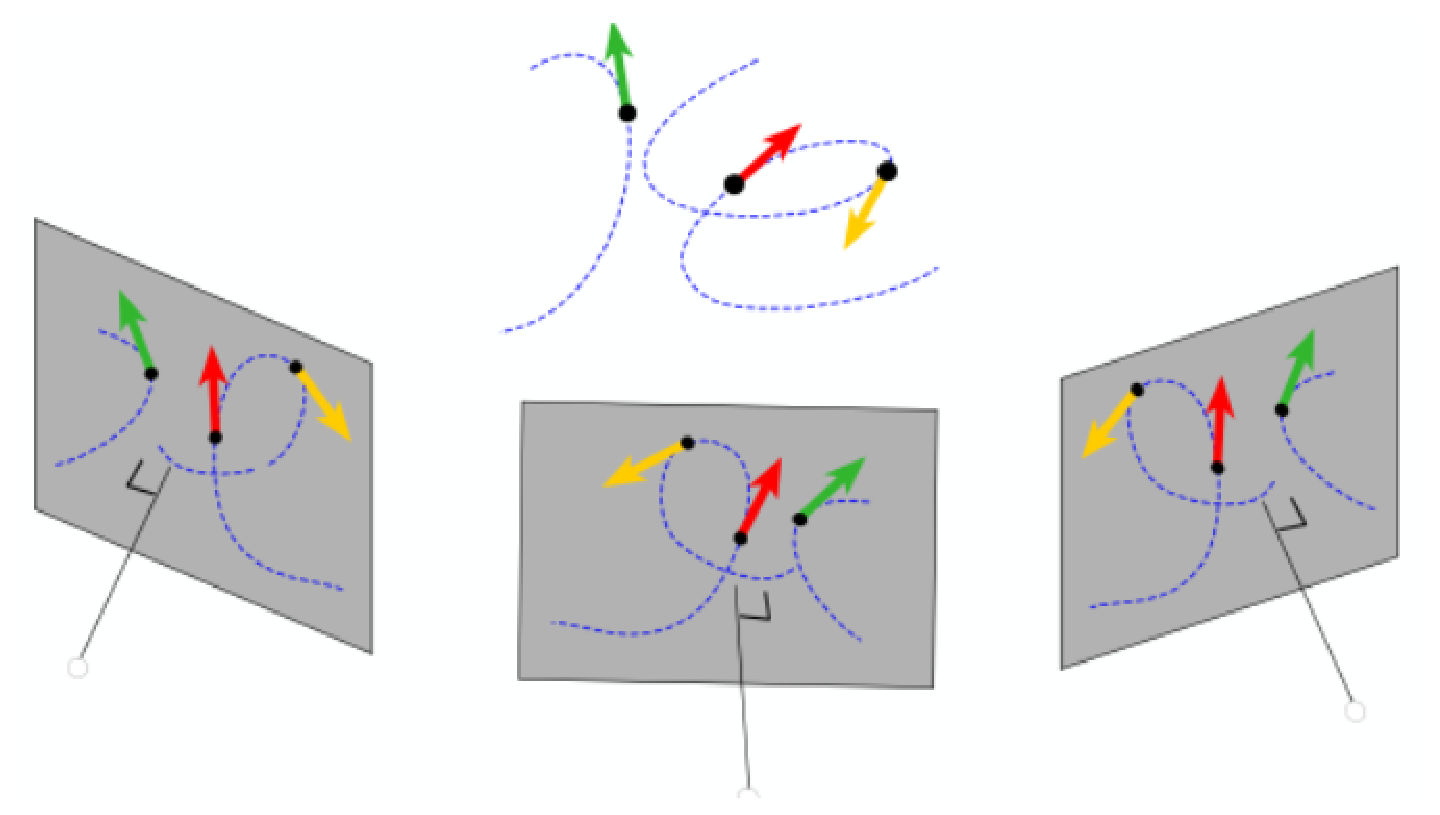
\includegraphics[scale=.45]{figuras/dife-tri}
\end{figure}
}
\section{Geometria trifocal calibrada}
\frame{\frametitle{Teorema 1: homografia de retas epipolares}
\begin{figure}[!htb]
\centering
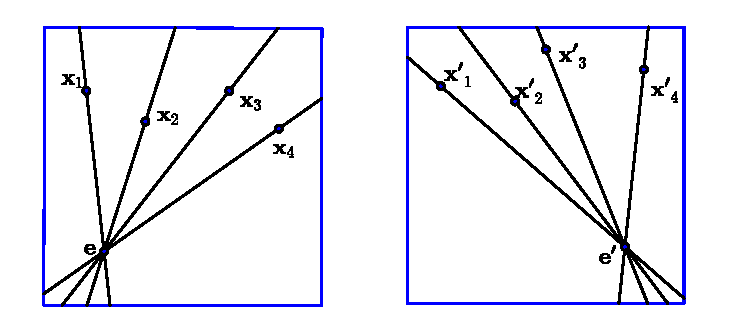
\includegraphics[scale=1]{figuras/retas-epipolares}
\end{figure}
\begin{equation*}
\lightrgb'=F\,[\e]_\times\,\lightrgb
\end{equation*}
}
%
%\frame{\frametitle{Teorema 1: homografia de retas epipolares}
%\begin{minipage}{.6\textwidth}
%\begin{equation*}
%{\bf m}\times\lightrgb=\x\qquad\text{ou}\qquad\,[{\bf m}]_\times\,\lightrgb=\x
%\end{equation*}
%\begin{equation*}
%\lightrgb'=F\,\x
%\end{equation*}
%\end{minipage}
%\begin{minipage}{.3\textwidth}
%\begin{equation*}
%\lightrgb'=F\,[{\bf m}]_\times\,\lightrgb
%\end{equation*}
%\begin{equation*}
%\lightrgb'=F\,[\e]_\times\,\lightrgb
%\end{equation*}
%\end{minipage}
%\begin{figure}[!htb]
%\centering
%\includegraphics[scale=.4]{figuras/reta-epipo-2}
%\end{figure}
%}
%
\frame{\frametitle{Teorema 2: restrições Kruppa}
\begin{minipage}{.5\textwidth}
\begin{equation*}
{\bf \omega}=K^{-\top}K^{-1}
\end{equation*}
\begin{equation*}
\omega^*=\omega^{-1}=K\,K^\top
\end{equation*}
\end{minipage}
\begin{minipage}{.4\textwidth}
\begin{equation*}
D=[\e]_\times\,{\bf \omega}^*\,[\e]_\times 
\end{equation*}
\begin{equation*}
D'=[\e']_\times\,{{\bf \omega}^*}'\,[\e']_\times
\end{equation*}
\end{minipage}
\begin{figure}[!htb]
\centering
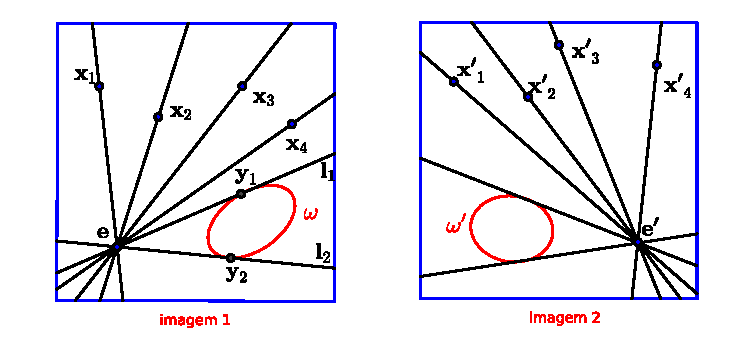
\includegraphics[scale=1]{figuras/restricao-epipolar-kruppa}
\end{figure}
}
%
%\frame{\frametitle{}
%\begin{equation*}
%\begin{array}{rcll}
%[\e']_\times\,{{\bf \omega}^*}'\,[\e']_\times&=&D'&\\
%&=&H_\infty^{-\top}D\,H_\infty^{-1}&\\
%&=&H_\infty^{-\top}[\e]_\times\,{\bf \omega}^*\,[\e]_\times\,H_\infty^{-1}&\qquad\text{pois}\qquad D=[\e]_\times\,{\bf \omega}^*\,[\e]_\times\\
%%&=&F\,\omega^* F^\top,&
%\end{array}
%\end{equation*}
%\begin{figure}[!htb]
%\centering
%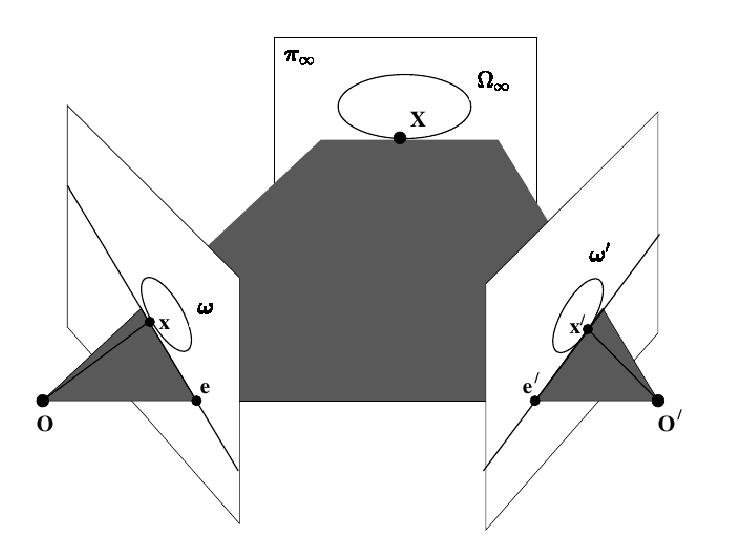
\includegraphics[scale=.8]{figuras/geometria-kruppa}
%\end{figure}
%}
%
\frame{\frametitle{Teorema 3: pontos e epipolos co-cônicos}
\begin{equation*}
\x'_i=H\,\x_i
\end{equation*}\\\quad\\
\begin{figure}[!htb]
\centering
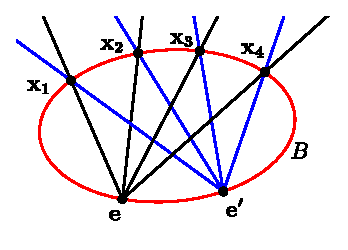
\includegraphics[scale=1.4]{figuras/pontos-conconicos}
\end{figure}
}
%
\frame{\frametitle{Teorema 4: restrições de calibração}
\begin{figure}[!htb]
\centering
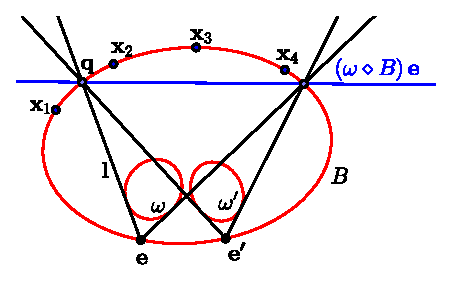
\includegraphics[scale=1.3]{figuras/projecao-omega-B}
\end{figure}
\begin{minipage}{1\textwidth}
As projeções de ${\bf \omega}$ e ${\bf \omega'}$ em $B$, através dos respectivos epipolos, devem coincidir.
\end{minipage}
}
%
\frame{\frametitle{Representação canônica de uma cônica}
\begin{equation*}
(\omega \diamond B)\equiv 2\,B\,\omega^*B - tr(\omega^*\,B)\,B
\end{equation*}
\begin{equation*}
B=
\begin{bmatrix}
0&0&1\\
0&-2&0\\
1&0&0
\end{bmatrix}
\qquad\text{e}\qquad
\omega^*=
\begin{bmatrix}
c_{11}&c_{12}&c_{13}\\
c_{12}&c_{22}&c_{23}\\
c_{13}&c_{23}&c_{33}
\end{bmatrix}
\end{equation*}
\begin{equation*}
\begin{pmatrix}
1&\theta&\theta^2
\end{pmatrix}
\begin{bmatrix}
0&0&1\\
0&-2&0\\
1&0&0
\end{bmatrix}
\begin{pmatrix}
1\\
\theta\\
\theta^2
\end{pmatrix}
=0
\end{equation*}
\begin{figure}[!htb]
\centering
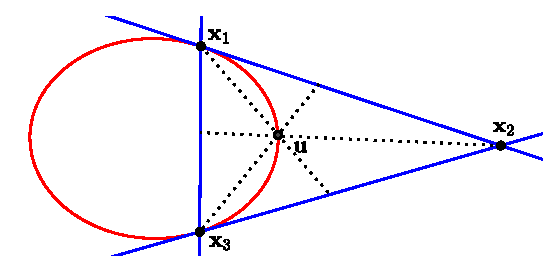
\includegraphics[scale=.9]{figuras/conica-tri-referencia}
\end{figure}
}
%
\frame{\frametitle{Teorema 5 e 6: restriç\~oes de projeção}
\begin{figure}[!htb]
\centering
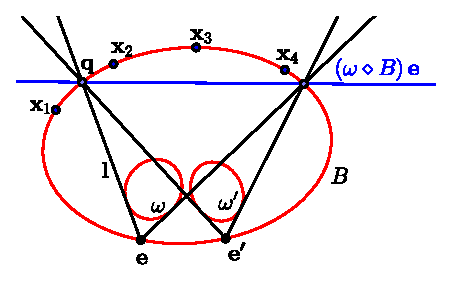
\includegraphics[scale=1.3]{figuras/projecao-omega-B}
\end{figure}
\begin{minipage}{1\textwidth}
$(\omega\diamond B)\,\e$\quad e\quad $(\omega'\diamond B)\,\e'$\quad coincidem
\end{minipage}
}
%
\frame{\frametitle{Teorema 7: a função que relaciona os epipolos}
\begin{minipage}{.5\textwidth}
\begin{equation*}
(\omega \diamond B)\equiv 2\,B\,\omega^*B - tr(\omega^*\,B)\,B
\end{equation*}
\begin{center}
$(\omega \diamond B) = B\,(\omega \cdot B)$
\end{center}
\end{minipage}
\begin{minipage}{.4\textwidth}
\begin{equation*}
(\omega \cdot B) \equiv 2\,\omega^*\,B - tr(\omega^*\,B)\,I
\end{equation*}
\begin{equation*}
B(\e)=(\e^\top B_2\e)\,B_1-(\e^\top B_1\e)\,B_2
\end{equation*}
\end{minipage}
\begin{figure}[!htb]
\centering
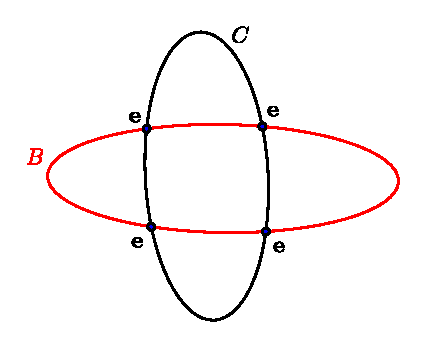
\includegraphics[scale=.7]{figuras/intersecao-C-B}
\end{figure}
\begin{equation*}
{\bf e} \rightarrow {\bf e'} \sim (\omega' \cdot B)^*\,(\omega \cdot B)\,{\bf e}
\end{equation*}
\begin{equation*}
C \equiv (\omega \cdot B)^\top\,(\omega' \cdot B)^{*\,\top}\,B\,(\omega' \cdot B)^*(\omega \cdot B)
\end{equation*}
}
%
\frame{\frametitle{Redução de $C$ a $G$}
\begin{minipage}{.5\textwidth}
\begin{center}
$\e^\top C\,\e=0$
\end{center}
\end{minipage}
\begin{minipage}{.4\textwidth}
\begin{equation*}
\e^\top\,G\,\e=0
\end{equation*}
\end{minipage}
\begin{equation*}
G=4\,U^\top D'^*\,B^*\,D'^*\,U-4\,t'^2\,B\,D\,D'^*\,(D\,B-t\,I)+s\,D^*-t^2\,t'^2\,D'^*
\end{equation*}
\begin{equation*}
\begin{array}{rcl}
D&\equiv&\omega^*,\\
t&\equiv&tr(D\,B),\\
U&\equiv&(\omega \cdot B)\,\,\, \text{e}\\
s&=&(16\,|B|\,|D'|\,t'+t'^4-4\,t'^2\,tr(B^*\,D'^*)).
\end{array}
\end{equation*}
\begin{figure}[!htb]
\centering
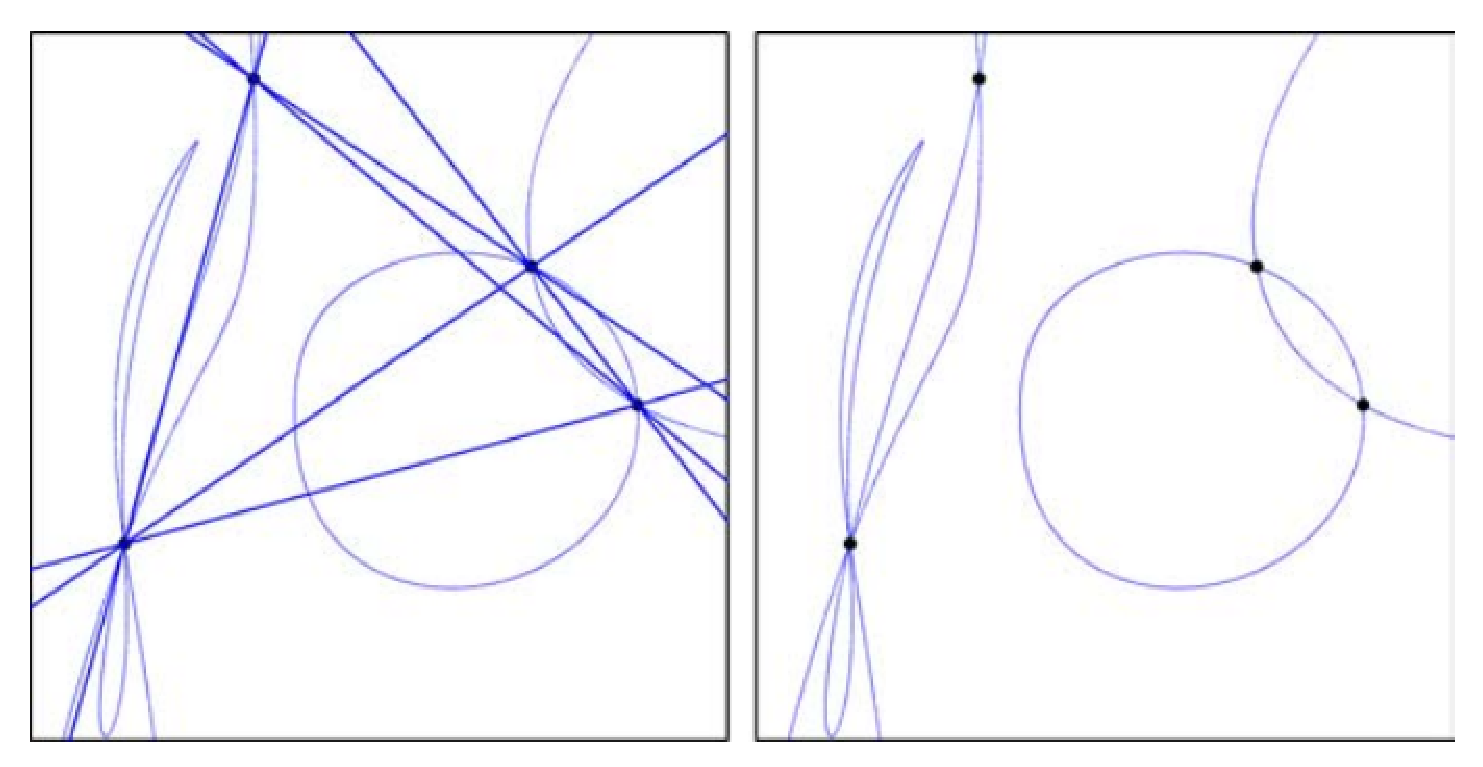
\includegraphics[scale=.35]{figuras/plotagem-C}
\end{figure}
}
%
\frame{\frametitle{Resumo do algoritmo}
\begin{enumerate}
\item $x\leftrightarrow x'$ determinar $H$\vspace{.15 cm}
\item $\e=(1,\theta,\theta^2)^\top$\vspace{.15 cm}
\item $B(e)=(\e^\top B_2\e)\,B_1-(\e^\top B_1\e)\,B_2,$\vspace{.15 cm}
\item $\omega=K^{-\top}K^{-1}$\vspace{.15 cm}
\item $B$, $\omega$ e $\omega^*$ determinar $G$\vspace{.15 cm}
\item quatro soluções para ${\bf e}$ (ap\^endice A)\vspace{.15 cm}
\item quatro soluções para ${\bf e'}$ (apêndice B)\vspace{.15 cm}
\item homografia $\longrightarrow$ matriz essencial\vspace{.15 cm}
\item câmeras $\longrightarrow$ reconstrução dos quatro pontos 3D\vspace{.15 cm}
\item abordagem de Kuang e {\AA}str{\"o}m [2013]
\end{enumerate}
}
%
\frame{\frametitle{Conclus\~oes e trabalhos futuros}
\begin{enumerate}
\item coordenadas homog\^eneas, transla\c{c}\~ao, normaliza\c{c}\~ao por divis\~ao, objetos geométrico-algébricos abstratos \vspace{.15 cm}
\item aux\'ilio de outras áreas da matemática\vspace{.15 cm}
\item benefícios te\'oricos do tensor trifocal\vspace{.15 cm}
\item complexidade da tarefa de se determinar as três câmeras num sistema trifocal\vspace{.15 cm}
\item trabalhos futuros
\end{enumerate}
}
%
\frame{\frametitle{}
\begin{center}
\textcolor{blue}{\large{OBRIGADO}}
\end{center}
}
\end{document}\grid
